\chapter{Further work on the model}
\label{secondPhaseOfModelingCyberInsurance} 

So far our model have only considered the affects from direct connections. Now we are introducing a way of analyzing how network formation will  be affected from indirect connections. 

In the previous models the utility equation for each node have only been affected by direct variables such as $\beta$. In a real world scenario a node will be strongly affected by network externalities. Our idea is based on the paper from Jackson and Wolinsky \cite{jackson1996strategic} and a network formation game in \cite{jackson2005survey}. 

\section{The connection game}
We consider a connection game which reflects not only the benefit from establishing connections to other people, but also the benefits from indirect connections. Meaning, in addition to the benefit from the direct connection, a node will also benefit from "a friend of a friend", although the benefit will be a factor lower than the direct connection, also "friends of a friend of a friend" will generate benefit and so forth. The payoff will be calculated relative to the distance between different nodes.


\begin{figure}[h]
\centering
  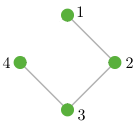
\includegraphics[width=0.2\linewidth]{../Figures/connectionGame.png}
  \caption{\label{fig:connectionGame} Four nodes interconnected with each other.}
\end{figure}
For instance, node 1 in the network depicted in figure \ref{fig:connectionGame}, will benefit $\beta$ from node 2, $\beta^{2}$ from node 3 and $\beta^{3}$ from node 4. The benefit will decrease relative to the shortest path between two nodes as long as $\beta < 1$. Hence the payoff a node receives from the network equals: 

\begin{equation}
\sum_{j\neq i}^{} \beta_{ij}^{d(ij)} - \sum_{j:ij\in g}^{} {I_{l}}_{ij}, 
\label{connecetionGame}
\end{equation}

where $d(ij)$ represents the shortest path between node $i $ and node $j $, and ${I_{l}}_{ij}$ represents node i's cost of insuring a link between the two nodes. To simplify the model we choose a symmetric connection process where $\beta$ and $I_{l}$ is set to a fixed global value. 

To analyze the different outcomes of the game, one might consider making the network as efficient as possible or focus on creating a stable network. An efficient network means ending up with a network which generates the most total value for the players. Intuitively, this network is preferable if it is stable. However, as we shall see there might be some conflict areas between efficiency and stability. 

The paper from \cite{jackson1996strategic} showed that the following propositions for analyzing the game as an efficient network structure:
\begin{enumerate}
\item \textit{a complete graph $g^N$ if $I_{l}<\beta - \beta^2$,}
\item \textit{a star encompassing every node if $\beta - \beta^2 < i_{l} < \beta + \frac{(N-2)}{2}\beta^2$,}
\item \textit{no links if $\beta + \frac{(N-2)}{2}\beta^2 < I_{l}$.}
\end{enumerate}

Generally it means that when the cost of insuring a link is low, it would be more beneficial to have a direct connection to a node than indirectly benefiting from it. When the insurance cost is high, it would not be more beneficial not to establish any connections at all.
The most efficient structure is created in the intermediate cost of insuring links, and ends up in a star structure which encompasses every node. A star structure have the characteristics of minimizing the average path length and uses only a minimal number of links. Indisputable this structure provides the highest overall payoff for the network, however, this network is not stable.
The reason is because the center node of the star will bear the cost of insuring every link connected, which generates a huge cost compared to the other nodes. This scenario is quite unfair, since the center node generates a great deal of network externalities for the other nodes, without being compensated. Hence a number of connections to the center node will not be pairwise stable, and the network will not be stable. 

The conditions has to be changed in order to met the requirements for stability, Jackson and Wolinsky presents the following proposition:

\begin{enumerate}

\item \textit{a pairwise stable network consists of at most one (non-empty) component,}
\item \textit{if $I_{l}<\beta - \beta^2$, the unique pairwise stable network will be a complete graph $g^N$, }
\item \textit{if $\beta - \beta^2 < I_{l} < \beta $, a star encompassing every node will be pairwise stable, although not unique,}
\item \textit{if $\beta < I_{l}$, any pairwise stable network which is nonempty is such that each player has at least two links and thus be inefficient. }
\end{enumerate}

As we can see, the conditions for high and low insurance cost is similar to the previous outcome in the efficient network structure. In addition, the case of intermediate insurance cost will become a stable network, since every new link connected will result in a higher payoff, due to $I_{l} < \beta$. However, it should be noticed that it would be more beneficial for a node to operate at a leaf node in the network, instead of being a center node, due to the cost of insuring each new link. In a perfect star structure, a leaf node will only have to insure the node to the center node, and will benefit indirectly for each node connected to the center node. The center node will benefit from each new connection, however, the payoff will only be $\beta - I{l}$ for each connection. Therefore it is desirable to be a leaf node. 

To solve the problem, one has to compensate the center node for the extra cost of creating network externalities. As described in the previous model considering bulk insurance discount, the insurance company could implement a bonus which lowers the cost for each new connection. This would lower the extra cost for the center node significantly, as it is expected that the number of nodes might be high and therefor result in a significant discount. 
Using the discount calculation from previous models, we end up with the following equation for the star topology:

\begin{equation}
\beta-\beta^2<\frac{i_{l}}{i+1}< \beta
\end{equation}



where $i $ is represent the number of connections a node have established. 

Although this enhancement ensures that the cost for the center node is lowered, it does not guarantee that the center node is fully compensated. To accomplish this, the insurance companies have to directly compensate the center nodes. As described earlier a star topology will create a super critical payoff, and a star topology would be beneficial for the insurance companies. Hence the insurance companies will have incentive to compensate the center nodes additionally to enable the star structure to be generated. 

input{modelFromBohme}

